\section{Environment descriptions and visualizations}

The following figures show and describe MDVDRPs in general, as well as particular visualizations for all dispatching environments. 

\begin{figure}[H]
\begin{floatrow}
\centering
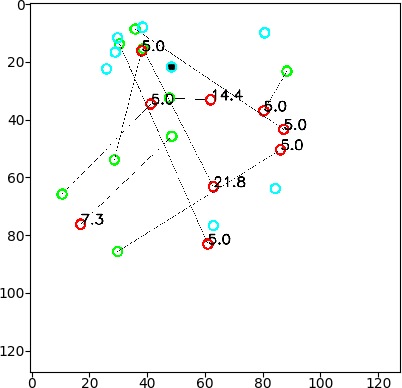
\includegraphics[width=.75\linewidth]{sections/mddqn/figures/policy_5min_cropped.png}\label{fig:simulacrum}
\caption{A visual representation of a dispatching state. Blue dots represent drivers. The black centered driver located at position (60, 20) is available, and all others are dispatched. Orders start at red dots and end at the connected green dot. Order prices are denoted above their pickup location}
\end{floatrow}
\end{figure}

\begin{figure}[H]
\begin{floatrow}
\centering
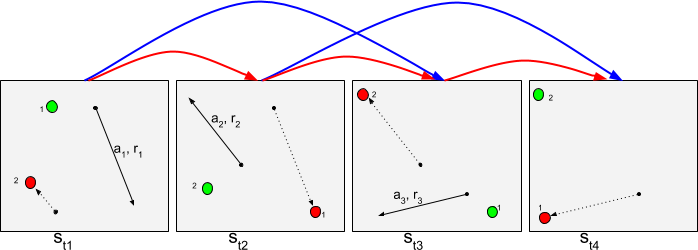
\includegraphics[width=1.\linewidth]{sections/mddqn/figures/dqn_state_transitions_cropped.png}\label{fig:dqn_trans}
\caption{The above image shows a length 4 trajectory. The currently available driver is green, dispatched driver is red, and the order that the available driver accepts at time $t_i$ is $a_i$ and has price $r_i$. The accepted order at time $t_i$ is labeled by its action name and price, $(a_i, r_i)$ and travels from the solid black dot to the terminal arrow. SD-DQN transitions are indicated by blue arrows above state, e.g. transition $(s_{t1}, a_1, r_1, s_{t3})$, which is driver-centric with respect to driver 1. MD-DQN transitions are indicated by red arrows e.g. transition$(s_{t1}, a_1, r_1, s_{t2})$, which transitions from a state where driver 1 is available to a state where driver 2 is available.}
\end{floatrow}
\end{figure}

\begin{figure}[H]
\begin{floatrow}
\centering
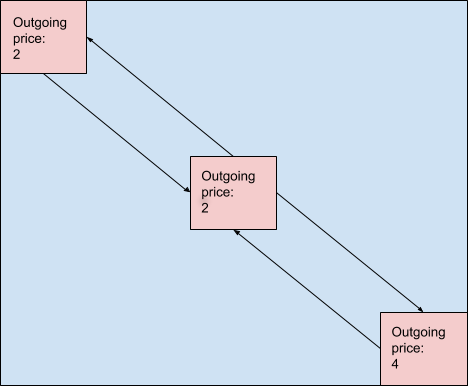
\includegraphics[width=.75\linewidth]{sections/mddqn/figures/Bonus_cropped.png}
\caption{Surge domain. Orders travel between the three red squares. Each square is labeled with its outgoing order value. Within each square, order start and end locations are generated uniformly randomly.}
\label{fig:surge}
\end{floatrow}
\end{figure}


\begin{figure}[H]
\begin{floatrow}
\centering
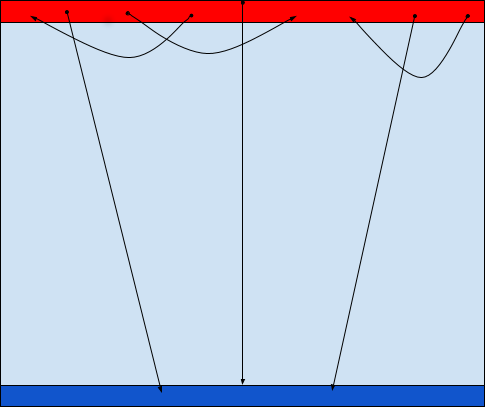
\includegraphics[width=.75\linewidth]{sections/mddqn/figures/HotCold_cropped.png}
\caption{Hot/Cold domain. Orders all begin in the red bar, with their positions generated uniformly randomly. For the destination, a fair coin is flipped to decide whether the order ends in hot or cold, and then the exact position is sampled uniformly randomly in the designated region.}
\label{fig:hc}
\end{floatrow}
\end{figure}

\begin{figure}[H]
\begin{floatrow}
\centering
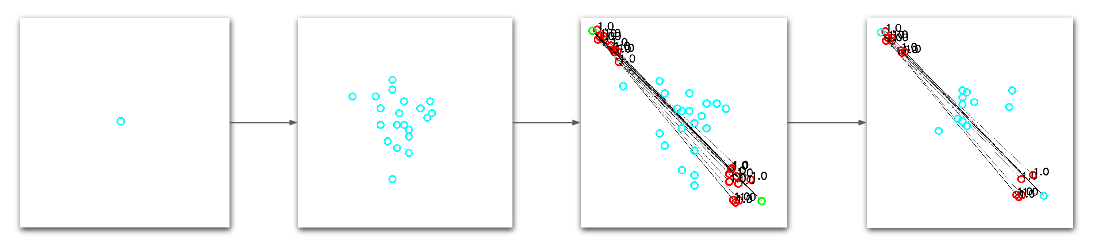
\includegraphics[width=.75\linewidth]{sections/mddqn/figures/distribute_domain.png}\label{fig:distribute}
\caption{Distribute domain. Drivers begin in the center of the region. They then proceed with 5 steps of repositioning. At the $6^{th}$ timestep, orders appear in the two corners. Drivers that are within .3 units of an order start, denoted by a red circle, are assigned. All orders end in the opposing corner’s green dot so that trips are long enough that a single driver can only satisfy one order per episode. After two timesteps, all remaining orders cancel and the environment resets.}
\end{floatrow}
\end{figure}

\begin{figure}[H]
\begin{floatrow}
\centering
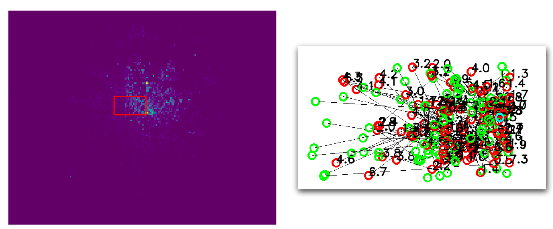
\includegraphics[width=.75\linewidth]{sections/mddqn/figures/historic_simulator.png}\label{fig:historic}
\caption{Historic data order start distribution and corresponding simulator rendering. The red box indicates the spatial region that is selected for the simulator. an average of 10 percent of orders start and end in this region, which roughly correspond to an edge of downtown and some outlying areas.}
\end{floatrow}
\end{figure}


\subsection{Graphs}
In the following graphs, the units of the x-axis are in {\em episodes}. For the nonrepositioning illustrative domains, an episode lasts 5000 time units. In the Repositioning Hot/Cold domain an episode is 500 time units. The distribute domain lasts 7 time units. The realistic domains last for 1440 time units in the realistic simulator. Graphs for Distribute domains show served percentage on the y-axis, while all other curves are environment reward.

% \begin{figure}[H]
% \begin{floatrow}
% \centering
% \subfloat[]{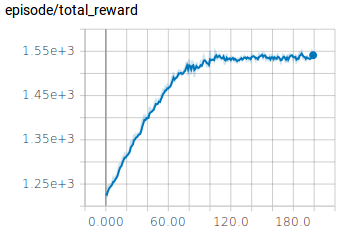
\includegraphics[width=.32\linewidth]{score3pREG.png}\label{fig:bonus}}

% \subfloat[]{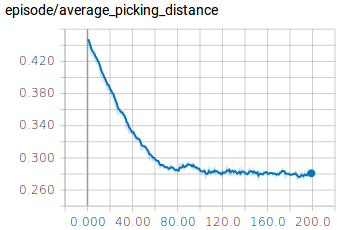
\includegraphics[width=.32\linewidth]{pd3pREG.png}}

% \subfloat[]{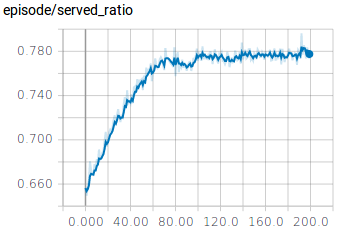
\includegraphics[width=.32\linewidth]{served3pREG.png}}
% \caption{SD-DQN on low-demand Surge domain}
% \end{floatrow}
% \end{figure}

% \begin{figure}[H]
% \begin{floatrow}
% \centering
% \subfloat[]{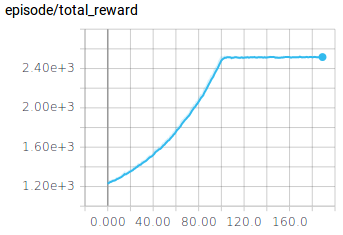
\includegraphics[width=.32\linewidth]{score10pREG.png}\label{fig:bonus}}

% \subfloat[]{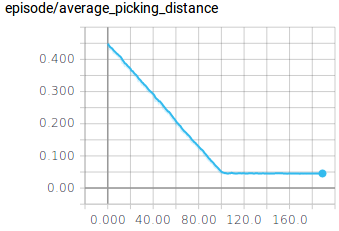
\includegraphics[width=.32\linewidth]{pd10pREG.png}}

% \subfloat[]{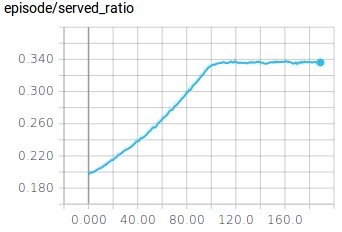
\includegraphics[width=.32\linewidth]{served10pREG.png}}
% \caption{SD-DQN on high-demand Surge domain}
% \end{floatrow}
% \end{figure}

% \begin{figure}[H]
% \begin{floatrow}
% \centering
% \subfloat[]{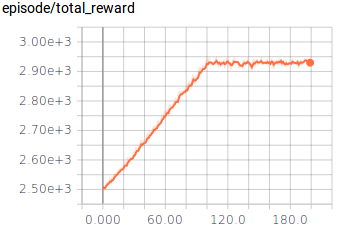
\includegraphics[width=.32\linewidth]{score3pHC.png}\label{fig:bonus}}

% \subfloat[]{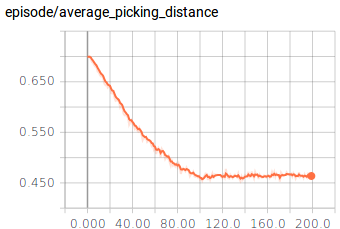
\includegraphics[width=.32\linewidth]{pd3pHC.png}}

% \subfloat[]{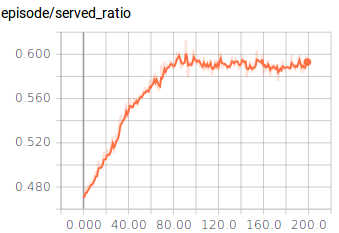
\includegraphics[width=.32\linewidth]{served3pHC.png}}
% \caption{SD-DQN on low-demand Hot/Cold domain}
% \end{floatrow}
% \end{figure}

% \begin{figure}[H]
% \begin{floatrow}
% \centering
% \subfloat[]{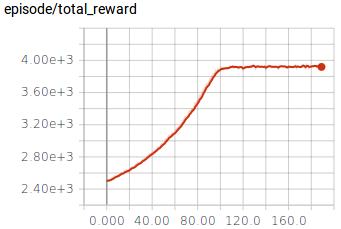
\includegraphics[width=.32\linewidth]{score10pHC.png}\label{fig:bonus}}

% \subfloat[]{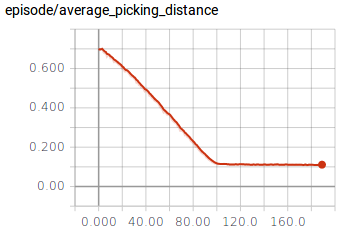
\includegraphics[width=.32\linewidth]{pd10pHC.png}}

% \subfloat[]{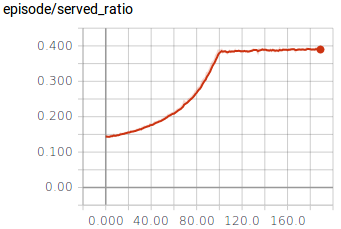
\includegraphics[width=.32\linewidth]{served10pHC.png}}
% \caption{SD-DQN on high-demand Hot/Cold domain}
% \end{floatrow}
% \end{figure}

% \begin{figure}[H]
% \begin{floatrow}
% \centering
% \subfloat[]{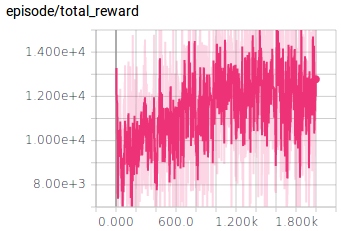
\includegraphics[width=.32\linewidth]{score01percent.png}\label{fig:bonus}}

% \subfloat[]{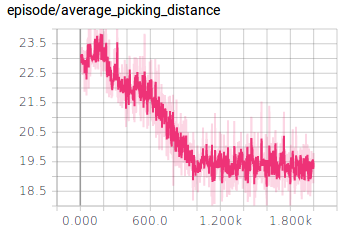
\includegraphics[width=.32\linewidth]{pd01percent.png}}

% \subfloat[]{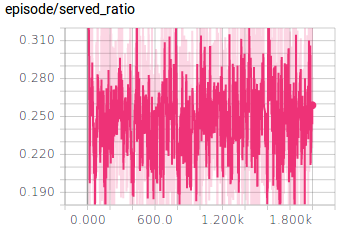
\includegraphics[width=.32\linewidth]{served01percent.png}}
% \caption{SD-DQN on .1\% real data simulator}
% \end{floatrow}
% \end{figure}

% \begin{figure}[H]
% \begin{floatrow}
% \centering
% \subfloat[]{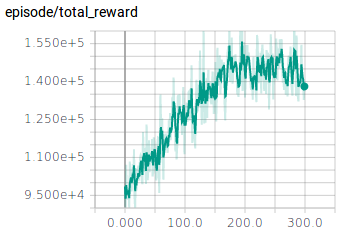
\includegraphics[width=.32\linewidth]{score1percent.png}\label{fig:bonus}}

% \subfloat[]{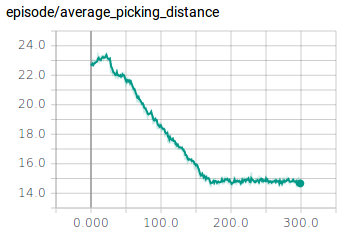
\includegraphics[width=.32\linewidth]{pd1percent.png}}

% \subfloat[]{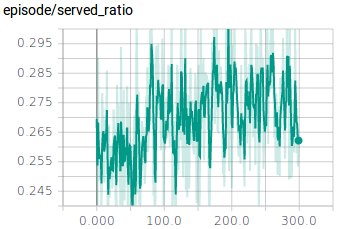
\includegraphics[width=.32\linewidth]{served1percent.png}}
% \caption{SD-DQN on 1\% real data simulator}
% \end{floatrow}
% \end{figure}

\begin{figure}[H]
\begin{floatrow}
\centering
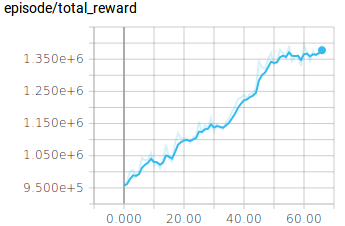
\includegraphics[width=1.0\linewidth]{sections/mddqn/figures/score10percent.png}\label{fig:10pscore}

% \subfloat[]{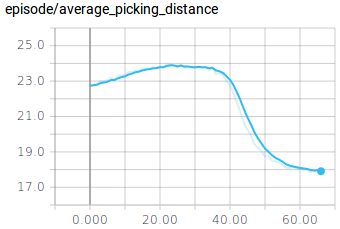
\includegraphics[width=.32\linewidth]{pd10percent.png}}

% \subfloat[]{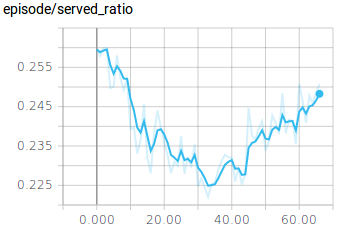
\includegraphics[width=.32\linewidth]{served10percent.png}}
\caption{SD-DQN on 10\% historical statistics simulator}
\end{floatrow}
\end{figure}

\subsection{Distribute Domains}

\begin{figure}[H]
\begin{floatrow}
\centering
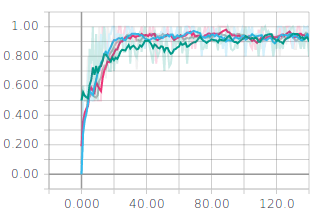
\includegraphics[width=1.0\linewidth]{sections/mddqn/figures/SDDQN_bal.png}\label{fig:balancedSD}

\caption{SDDQN served percentage on 20 driver 50/50 distribute domain}
\end{floatrow}
\end{figure}


\begin{figure}[H]
\begin{floatrow}
\centering
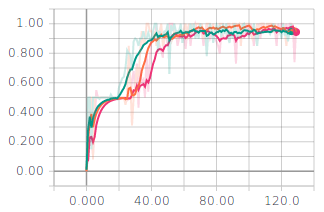
\includegraphics[width=1.0\linewidth]{sections/mddqn/figures/MDDQN_bal.png}\label{fig:balancedMD}

\caption{MDDQN served percentage on 20 driver 50/50 distribute domain}
\end{floatrow}
\end{figure}


\begin{figure}[H]
\begin{floatrow}
\centering
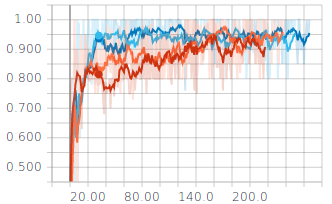
\includegraphics[width=1.0\linewidth]{sections/mddqn/figures/SDDQN_imbal.png}\label{fig:imbalancedSD}

\caption{SDDQN served percentage on 20 driver 80/20 distribute domain}
\end{floatrow}
\end{figure}


\begin{figure}[H]
\begin{floatrow}
\centering
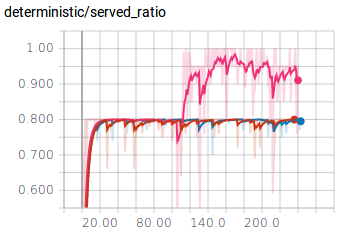
\includegraphics[width=1.0\linewidth]{sections/mddqn/figures/MDDQN_imbal2.png}\label{fig:imbalancedMD}

\caption{MDDQN served percentage on 20 driver 80/20 distribute domain}
\end{floatrow}
\end{figure}

\begin{figure}[H]
\begin{floatrow}
\centering
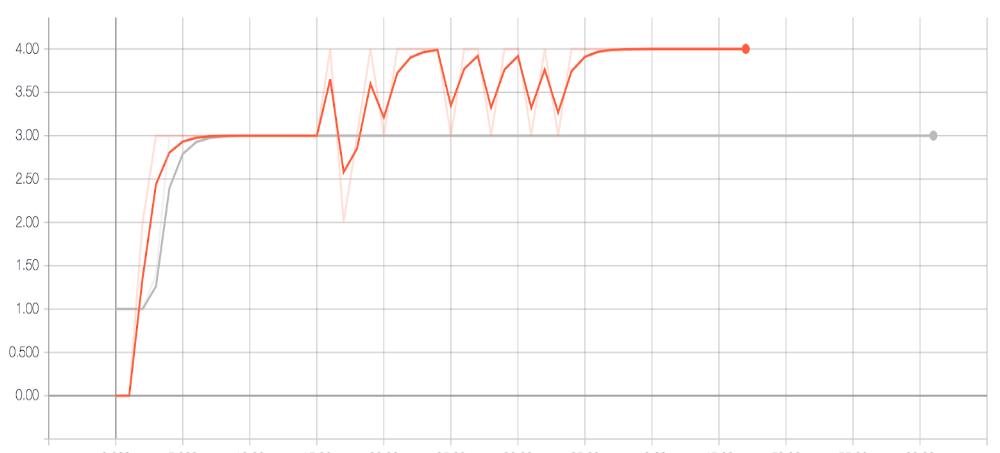
\includegraphics[width=1.0\linewidth]{sections/mddqn/figures/SDDQN_imbal4d.png}
\caption{SDDQN served percentage on 4 drivers 75/25 distribute domain. The orange curve shows SD-DQN performance when global context is included during the Q-value querying while the gray curve does not include global context. SDDQN without global context learns a policy that is uniform across drivers, and so it never escapes the uniform optimum.}
\label{fig:gs}
\end{floatrow}
\end{figure}






\subsection{Historical Data Domain}

\begin{figure}[H]
\begin{floatrow}
\centering
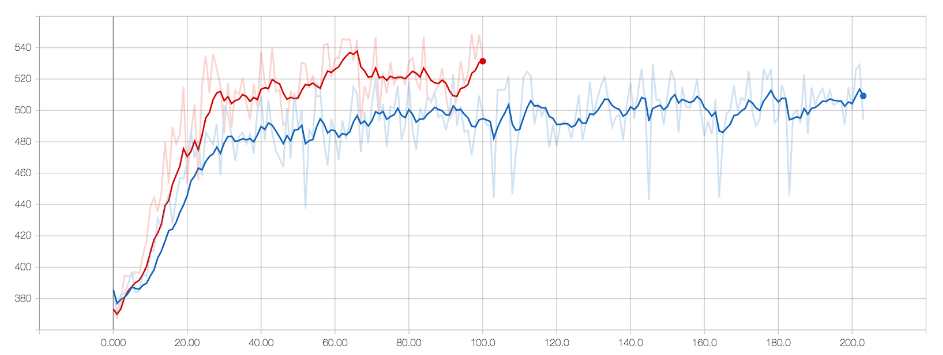
\includegraphics[width=1.0\linewidth]{sections/mddqn/figures/revenues.png}\label{fig:revenues}

\caption{SD-DQN revenue on 10\% historical simulator. The blue curve shows learning when revenue itself is used as the reward function. The red curve shows revenue when negative pickup distance is used as the reward function.}
\end{floatrow}
\end{figure}

\subsection{Training Details}

\subsubsection{20 Driver Static Assignment Problem}
 $\epsilon$-exploration is annealed linearly over $10,000$ episodes from 1.0 to 0.03, and the target network is updated every 500 training steps. The replay buffer maintains the $10000$ most recent transitions, and is initialized with $5000$ samples. We used a learning rate of $0.001$. Unlike the following domains, the reward function is given as the negative Euclidean distance between the selected driver-order pair.

\subsubsection{All other illustrative domains}
For SD-DQN we used a size 20000 replay buffer, learning rate 0.001, and we annealed $\epsilon$-exploration linearly over 100 episodes. We update the target network every 500 training updates, and perform a training update every environment step. For MD-DQN we used a size 20000 20-step Q-learning, a learning rate of 0.0001, and annealed $\epsilon$-exploration linearly over 100 episodes. We found it critical to stability to reduce the learning rate and perform $n$-step Q-learning in MD-DQN.
